\begin{figure}[htbp]
  \centering
  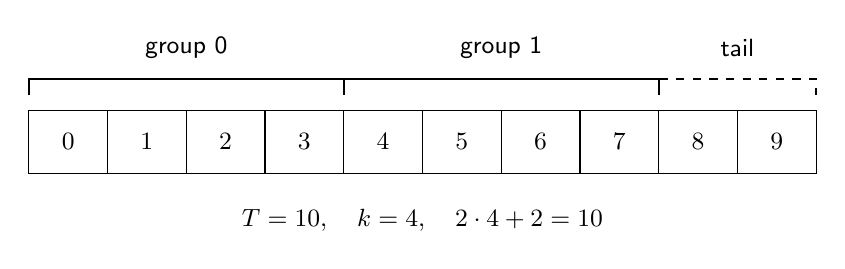
\begin{tikzpicture}[x=10mm,y=10mm]
    \foreach \i in {0,...,9} {
      \draw (\i,0) rectangle +(1,0.8);
      \node[font=\small] at (\i+0.5,0.4) {\i};
    }
    \draw[thick] (0,1) -- (0,1.2) -- (4,1.2) -- (4,1);
    \draw[thick] (4,1) -- (4,1.2) -- (8,1.2) -- (8,1);
    \draw[dashed,thick] (8,1) -- (8,1.2) -- (10,1.2) -- (10,1);
    \node[font=\sffamily\small] at (2,1.6) {group 0};
    \node[font=\sffamily\small] at (6,1.6) {group 1};
    \node[font=\sffamily\small] at (9,1.6) {tail};
    \node[font=\small] at (5,-0.6) {$T=10,\quad k=4,\quad 2\cdot4+2=10$};
  \end{tikzpicture}
  \caption{Two full groups and a two-iteration tail cover ten iterations once each, preserving their original order.}
  \label{fig:visual-unroll-tail}
\end{figure}
